\section{Introduction}\label{sec: Introduction}
The goal of final project is to familiarize the student with the groove connector and the possible interface methods provided with MicroBlaze and low level C code. The student will also write a software pulse width modulation (PWM). The outlined tasks are build on the PYNQ platform shown in Figure \ref{fig: intro1}. The MicroBlaze system is placed in between of the peripherals and the Zynq processing system (PS) as shown in Figure \ref{fig: intro2}. The MicroBlaze is in fact an from Xilinx developed softcore.

\begin{figure}[H]
	\centering
	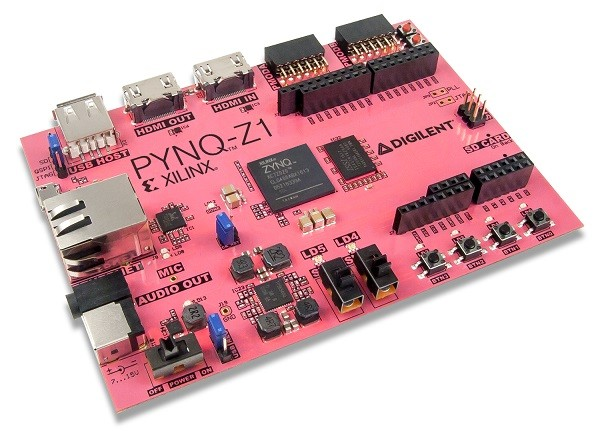
\includegraphics[width=0.6\textwidth]{01_images/PYNQ_Hardware_Xilinx}
	\caption{Xilinx PYNQ-Z1 development board SoC \cite{XUP}.}
	\label{fig: intro1}
\end{figure}
\begin{figure}[H]
	\centering
	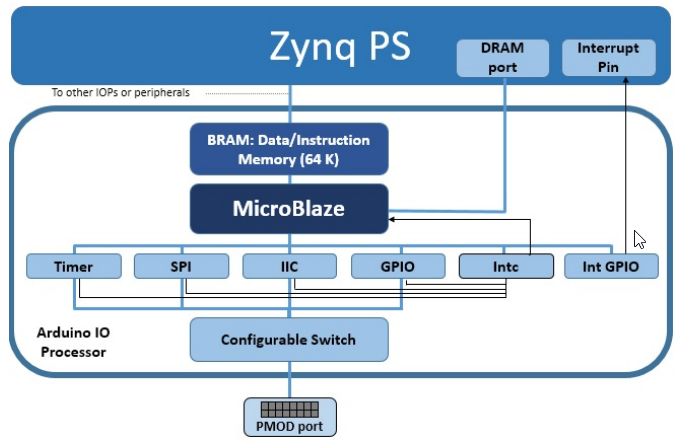
\includegraphics[width=0.8\textwidth]{01_images/PYNQ_Microblaze_Subsystem_Block_Diagram}
	\caption{PYNQ-Z1 block diagram of the MicroBlaze subsystem \cite{pynq_dr}.}
	\label{fig: intro2}
\end{figure}

